\subsection{Proof-of-Concept zur Veranschaulichung}
\label{sec:poc-methodology}

Die technische Machbarkeit der angedachten Architektur-Varianten aus \fullref{sec:traceability-architecture} soll exemplarisch mit einem \ac{poc} gezeigt werden. Es wird folgendesVorgehen angewendet.

\begin{enumerate}
    \item Definieren von didaktischen Kriterien
    \item Bewerten der Architektur-Varianten mit den Kriterien
    \item Beschreibung des Umfangs des \ac{poc} basierend auf der Architektur-Variante
\end{enumerate}

Die Wahl der Variante orientiert sich hierbei an didaktischen Kriterien und soll nicht die Evaluation der verschiedenen Architekturen aus \fullref{sec:evaluation} vorwegnehmen. Der Fokus liegt somit den grundlegenden Mechanismus der Traceability demonstrieren zu können und die Machbarkeit von zentralen Aspekten zu demonstrieren.

\begin{longtable}{|
  L{3cm}|
  p{\dimexpr\textwidth-8cm-6\tabcolsep-4\arrayrulewidth\relax}|
  L{5cm}|
}
    \hline
    \textbf{Kriterium} & \textbf{Beschreibung} & \textbf{Didaktische Relevanz} \\
    \hline
    \endfirsthead

    \hline
    \textbf{Kriterium} & \textbf{Beschreibung} & \textbf{Didaktische Relevanz} \\
    \hline
    \endhead

    Darstellung von Traceability Relationships &
    Die Architektur-Variante erlaubt eine verständliche Darstellung der Traceability-Beziehungen zwischen den regulatorischen Anforderungen und den architektonischen Artefakten des Metamodells. Die Bewertung erfolgt von 1 als unverständliche Darstellung bis 4 als verständliche Darstellung. 4 gilt als erstrebenswerte Ausprägung &
    Zur Demonstration sollten die Beziehungen klar sichtbar sein. Implizite Beziehungen oder Zusammenhänge machen die Versinnbildlichung abstrakter
    \\
    \hline

    Explizite Abbildung von Verantwortlichkeiten &
    Die Architektur-Variante veranschaulicht die Zuordnung von Verantwortlichkeiten in der Architektur und den beteiligten Rollen wie bspw. Akteure aus dem Use-Case Diagramm in \fullref{fig:traceability-use-cases}. Die Bewertung erfolgt von 1 als implizite Abbildung bis 4 als explizite Abbildung. 4 gilt als erstrebenswerte Ausprägung &
    Der Use-Case der Traceability basiert auf der Interaktion zwischen den verschiedenen Rollen. Sprich Identifizieren der Regulation, definieren der technischen Umsetzung und der Anwendung. Deshalb ist eine Sichtbarkeit von dieser Interaktion relevant zu demonstrieren
    \\
    \hline

    Reduzierte strukturelle Komplexität &
    Die Architektur-Variante soll eine begrenzte strukturelle Komplexität besitzen und sich auf wesentliche architektonische Konzepte der Traceability-Architektur / Metamodell beschränken. Die Bewertung erfolgt von 1 als hohe Komplexität und 4 als geringe Komplexität. 4 gilt als erstrebenswerte Ausprägung &
    Der \ac{poc} soll zur Beleuchtung der zentralen Konzepte dienen und kein \ac{mvp} sein. Durch eine reduzierte Komplexität ist die Traceability-Logik einfacher nachzuvollziehen
    \\
    \hline

    Alignment mit Traceability Use-Case &
    Die Architektur-Variante deckt den Traceability Use-Case ab, ohne für den Use-Case irrelevante Konzepte/Implementationen einzuführen. Die Bewertung erfolgt von 1 als aufwändige Abbildung bis 4 als pragmatische Abbildung. 4 gilt als erstrebenswerte Ausprägung &
    Der \ac{poc} soll durch die Fokussierung auf den Use-Case seinen Fokus behalten und somit nicht ausufern
    \\
    \hline
    \caption{Didaktische Kriterien für Auswahl der Variante der Traceability-Architecture für den \ac{poc}}
    \label{tab:didactic-poc-criteria}
\end{longtable}

Basierend auf den Kriterien und der Bewertungsskala wird die Bewertung der verschiedenen Architektur-Varianten gewählt. Die Skalen sind jeweils so definiert, dass 4 als erstrebenswerte Ausprägung gilt, was jedoch nicht bedeutet, dass diese erreichbar ist.

\begin{longtable}{|
  L{3cm}|
  L{2.5cm}|
  p{\dimexpr\textwidth-5.5cm-6\tabcolsep-4\arrayrulewidth\relax}|
}
    \hline
    \multicolumn{3}{|c|}{Bewertung \textit{Darstellung von Traceability-Beziehungen}} \\
    \hline
    \textbf{Kriterium} & \textbf{Bewertung} & \textbf{Begründung} \\
    \hline
    \endfirsthead

    \hline
    \multicolumn{3}{|c|}{Bewertung \textit{Darstellung von Traceability-Beziehungen}} \\
    \hline
    \textbf{Kriterium} & \textbf{Bewertung} & \textbf{Begründung} \\
    \hline
    \endhead

    Control-centric & 4 & Ideale Darstellung wegen dem Grundgedanken der Architektur-Variante die Anforderungen aus den Regulationen nach Controls zu gruppieren
    \\
    \hline

    Component-centric & 3 & Beziehungen sind darstellbar, aber leitet sich indirekt über die Struktur nach \ac{lz} Components ab. Sprich, man muss erst die Components verstehen und dann ergibt sich die Traceability
    \\
    \hline

    Category-centric & 2 & Beziehungen sind indirekt über die Kategorien und wiederum die \ac{lz} Components absehbar. Die schlechtere Sichtbarkeit ergibt sich direkt aus dem Design-Gedanken ein Bundling via \ac{lz} Kategorien zu machen. Dadurch, dass der Fokus auf dem Labeling nach Kategorien liegt ist es jedoch aus Sicht Projektverantwortlichen einfach nachzuvollziehen.
    \\
    \hline

    Provider-native & 1 & Die Nutzung von Provider-nativen Tools ermöglicht zwar theoretischen gesehen eine Darstellung der Traceability, jedoch nur wenn man die technischen Implementationen der Plattformen einbezieht. Dadurch ergibt sich eine hohe Implizität der Abbildung der Traceability-Beziehungen
    \\
    \hline
    \caption{Bewertung Kriterium \textit{Darstellung von Traceability Relationships} aus \fullref{tab:didactic-poc-criteria}}
    \label{tab:evaluating-didactic-criteria1}
\end{longtable}

\begin{longtable}{|
  L{3cm}|
  L{2.5cm}|
  p{\dimexpr\textwidth-5.5cm-6\tabcolsep-4\arrayrulewidth\relax}|
}
    \hline
    \multicolumn{3}{|c|}{Bewertung \textit{Explizite Abbildung von Verantwortlichkeiten}} \\
    \hline
    \textbf{Kriterium} & \textbf{Bewertung} & \textbf{Begründung} \\
    \hline
    \endfirsthead

    \hline
    \multicolumn{3}{|c|}{Bewertung \textit{Explizite Abbildung von Verantwortlichkeiten}} \\
    \hline
    \textbf{Kriterium} & \textbf{Bewertung} & \textbf{Begründung} \\
    \hline
    \endhead

    Control-centric & 4 & Verantwortlichkeiten sind direkt an Akteure gebunden. Compliance Officer mit Definition von Controls und Cloud-Experte mit technischer Umsetzung basierend auf den Controls
    \\
    \hline

    Component-centric & 3 & Verantwortlichkeiten werden über die technischen \ac{lz} Components geregelt. Die Verantwortung für die Components ist jedoch nicht eindeutig
    \\
    \hline

    Category-centric & 2 & Verantwortung ist abstrahiert über die \ac{lz} Kategorien. Die Akteure verschwinden somit hinter der Kategorie / Zuordnung ist nicht direkt ersichtlich
    \\
    \hline

    Provider-native & 1 & Durch Nutzung von Plattformmechanismen ist die Rolle des Compliance Officers in der Architektur quasi nicht mehr sichtbar. Bzw. die Wahrnehmung ist, dass eine Verschiebung hin zum Cloud-Experte stattfindet.
    \\
    \hline
    \caption{Bewertung Kriterium \textit{Explizite Abbildungen von Verantwortlichkeiten} aus \fullref{tab:didactic-poc-criteria}}
    \label{tab:evaluating-didactic-criteria2}
\end{longtable}


\begin{longtable}{|
  L{3cm}|
  L{2.5cm}|
  p{\dimexpr\textwidth-5.5cm-6\tabcolsep-4\arrayrulewidth\relax}|
}
    \hline
    \multicolumn{3}{|c|}{Bewertung \textit{Reduzierte strukturelle Komplexität}} \\
    \hline
    \textbf{Kriterium} & \textbf{Bewertung} & \textbf{Begründung} \\
    \hline
    \endfirsthead

    \hline
    \multicolumn{3}{|c|}{Bewertung \textit{Reduzierte strukturelle Komplexität}} \\
    \hline
    \textbf{Kriterium} & \textbf{Bewertung} & \textbf{Begründung} \\
    \hline
    \endhead

    Control-centric & 3 & Architektur hat klares Ordnungsprinzip mit den Controls. Gleichzeitig ist dadurch jedoch die Anzahl an Traceability-Beziehungen höher
    \\
    \hline

    Component-centric & 3 & Struktur ist technisch intuitiv wegen dem Fokus auf die \ac{lz} Components, womit aber die Traceability-Beziehungen auch über die Components laufen. Für ein Verständnis der Traceability muss somit die technische Beziehung verstanden werden.
    \\
    \hline

    Category-centric & 4 & Die \ac{lz} Kategorien bündeln viele Details, wodurch die Architektur übersichtlich wirkt. Diese Übersichtlichkeit wird jedoch durch Abstraktion im Hintergrund gewonnen
    \\
    \hline

    Provider-native & 2 & Strukturelle Komplexität der Provider-spezifischen Services erschweren ein einheitliches Ordnungsprinzip zu etablieren. Somit schwerer nachzuvollziehen
    \\
    \hline
    \caption{Bewertung Kriterium \textit{Reduzierte strukturelle Komplexität} aus \fullref{tab:didactic-poc-criteria}}
    \label{tab:evaluating-didactic-criteria3}
\end{longtable}

\begin{longtable}{|
  L{3cm}|
  L{2.5cm}|
  p{\dimexpr\textwidth-5.5cm-6\tabcolsep-4\arrayrulewidth\relax}|
}
    \hline
    \multicolumn{3}{|c|}{Bewertung \textit{Alignment mit Traceability Use-Case}} \\
    \hline
    \textbf{Kriterium} & \textbf{Bewertung} & \textbf{Begründung} \\
    \hline
    \endfirsthead

    \hline
    \multicolumn{3}{|c|}{Bewertung \textit{Alignment mit Traceability Use-Case}} \\
    \hline
    \textbf{Kriterium} & \textbf{Bewertung} & \textbf{Begründung} \\
    \hline
    \endhead

    Control-centric & 3 & Der Fokus auf die Controls bildet bereits einen wichtigen Teil der Use-Cases ab, da der Fokus vom Compliance Officer ebenfalls hauptsächlich auf der Anwendung der Controls liegt.
    \\ 
    \hline

    Component-centric & 3 & Der Fokus auf die \ac{lz} Components erfordert zuerst eine Ableitung über die technischen Components und erst anschliessend treten die Controls hervor, welche im Use-Case Ablauf beschrieben werden.
    \\
    \hline

    Category-centric & 2 & Die Usability welche durch die \ac{lz} Kategorisierung erreicht wird, sorgt bei der Abbildung für den Use-Case für eine starke Vereinfachung. Durch diese tritt die Traceability-Logik in den Hintergrund
    \\
    \hline

    Provider-native & 2 & Die Provider-spezifischen Implementierungen lenken den Fokus von der Abbildung der Traceability-Beziehungen und somit von den definierten Use-Cases weg.
    \\
    \hline
    \caption{Bewertung Kriterium \textit{Alignment mit Traceability Use-Case} aus \fullref{tab:didactic-poc-criteria}}
    \label{tab:evaluating-didactic-criteria4}
\end{longtable}

Basierend auf der Evaluation der Kriterien wird im \ac{poc} die Variante der Component-centric Architektur (Variante 2) verwendet. Eine weitere Überlegung zu den bereits evaluierten Kriterien ist, dass die Aufteilung in die \ac{lz} Komponenten gewissermassen auch einer Know-how Strukturierung bspw im \ac{bit} entsprechen könnte. Gemeint ist die Aufteilung bspw. in Networking, Storage, \ac{iam} etc, welche so die Annahme teilweise von verschiedene Abteilungen im \ac{bit} verantwortet werden. Der \ac{poc} soll somit zu der Funktionsweise der Traceability-Architecture zugleich die Abbildungen auf die verschiedenen Ausprägungen des Cloud-Experte (durch die verschiedenen Abteilungen) gerecht werden.

Der \ac{poc} soll einen Fokus auf die Traceability-Architecture gewährleisten. Der Scope erhebt somit nicht den Anspruch einer ganzheitlichen Implementierung, sondern dedizierte Aspekte hervorzuheben. Um gleichwohl im Sinne der didaktischen Ziele eine gute Veranschaulichung zu erhalten, wird ein GUI-Prototyp für die Komponente namens Governacne-Cockpit generiert. Dieser Prototyp (siehe \fullref{appendix:ui-mockup}) soll aufzeigen wie sich ein Tool für die Akteure aus \fullref{tab:uc6-verify-compliance} verhalten würde, welche auf einem System mit der Traceability-Architecture aufbaut. Das Ziel ist somit die Nutzerzentrierung, sprich den Fokus auf die Use-Cases der Organisation sicherzustellen. Die wesentlichen Schritte aus dem Hauptablauf des Use-Cases sind hierbei: die Auswahl des Projektes durch den Compliance Officer wie in \autoref{fig:methodology-project-healthcare-view} und die Überprüfung des Compliance-Status inkl. Trace wie in \autoref{fig:methodology-project-healthcare-view-evidence}. 

\begin{figure}[H]
    \centering
    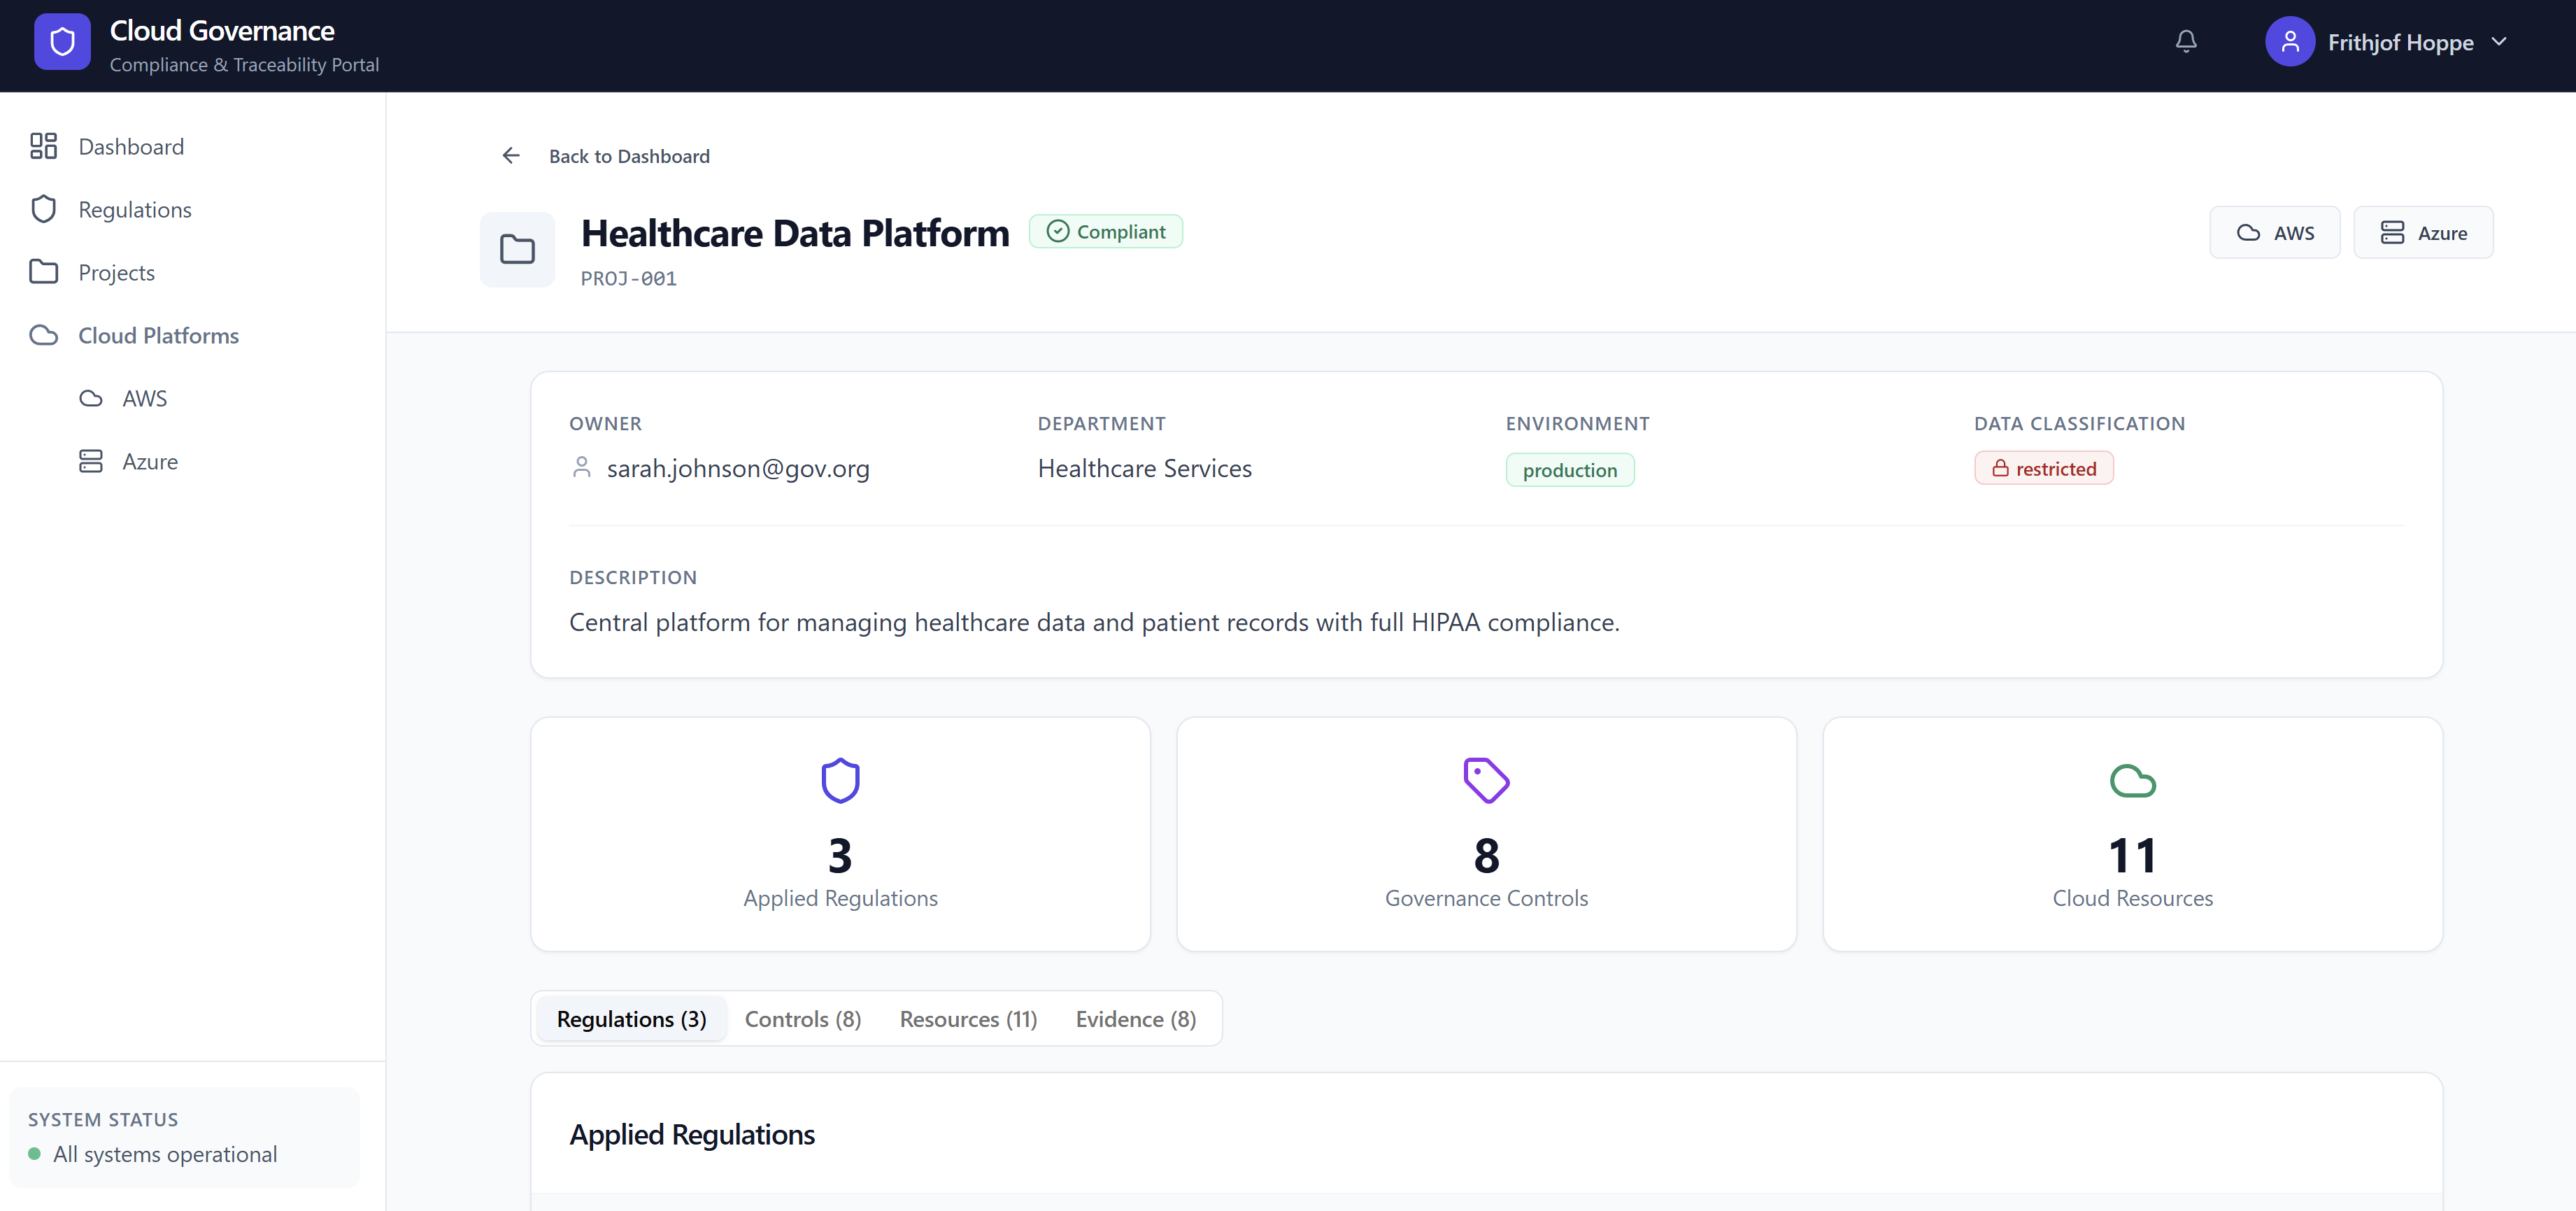
\includegraphics[width=0.8\textwidth]{graphics/ui-prototyp_project_healthcare.png}
    \caption{Detailansicht des Beispielprojekts Healthcare}
    \label{fig:methodology-project-healthcare-view}
\end{figure}

\begin{figure}[H]
    \centering
    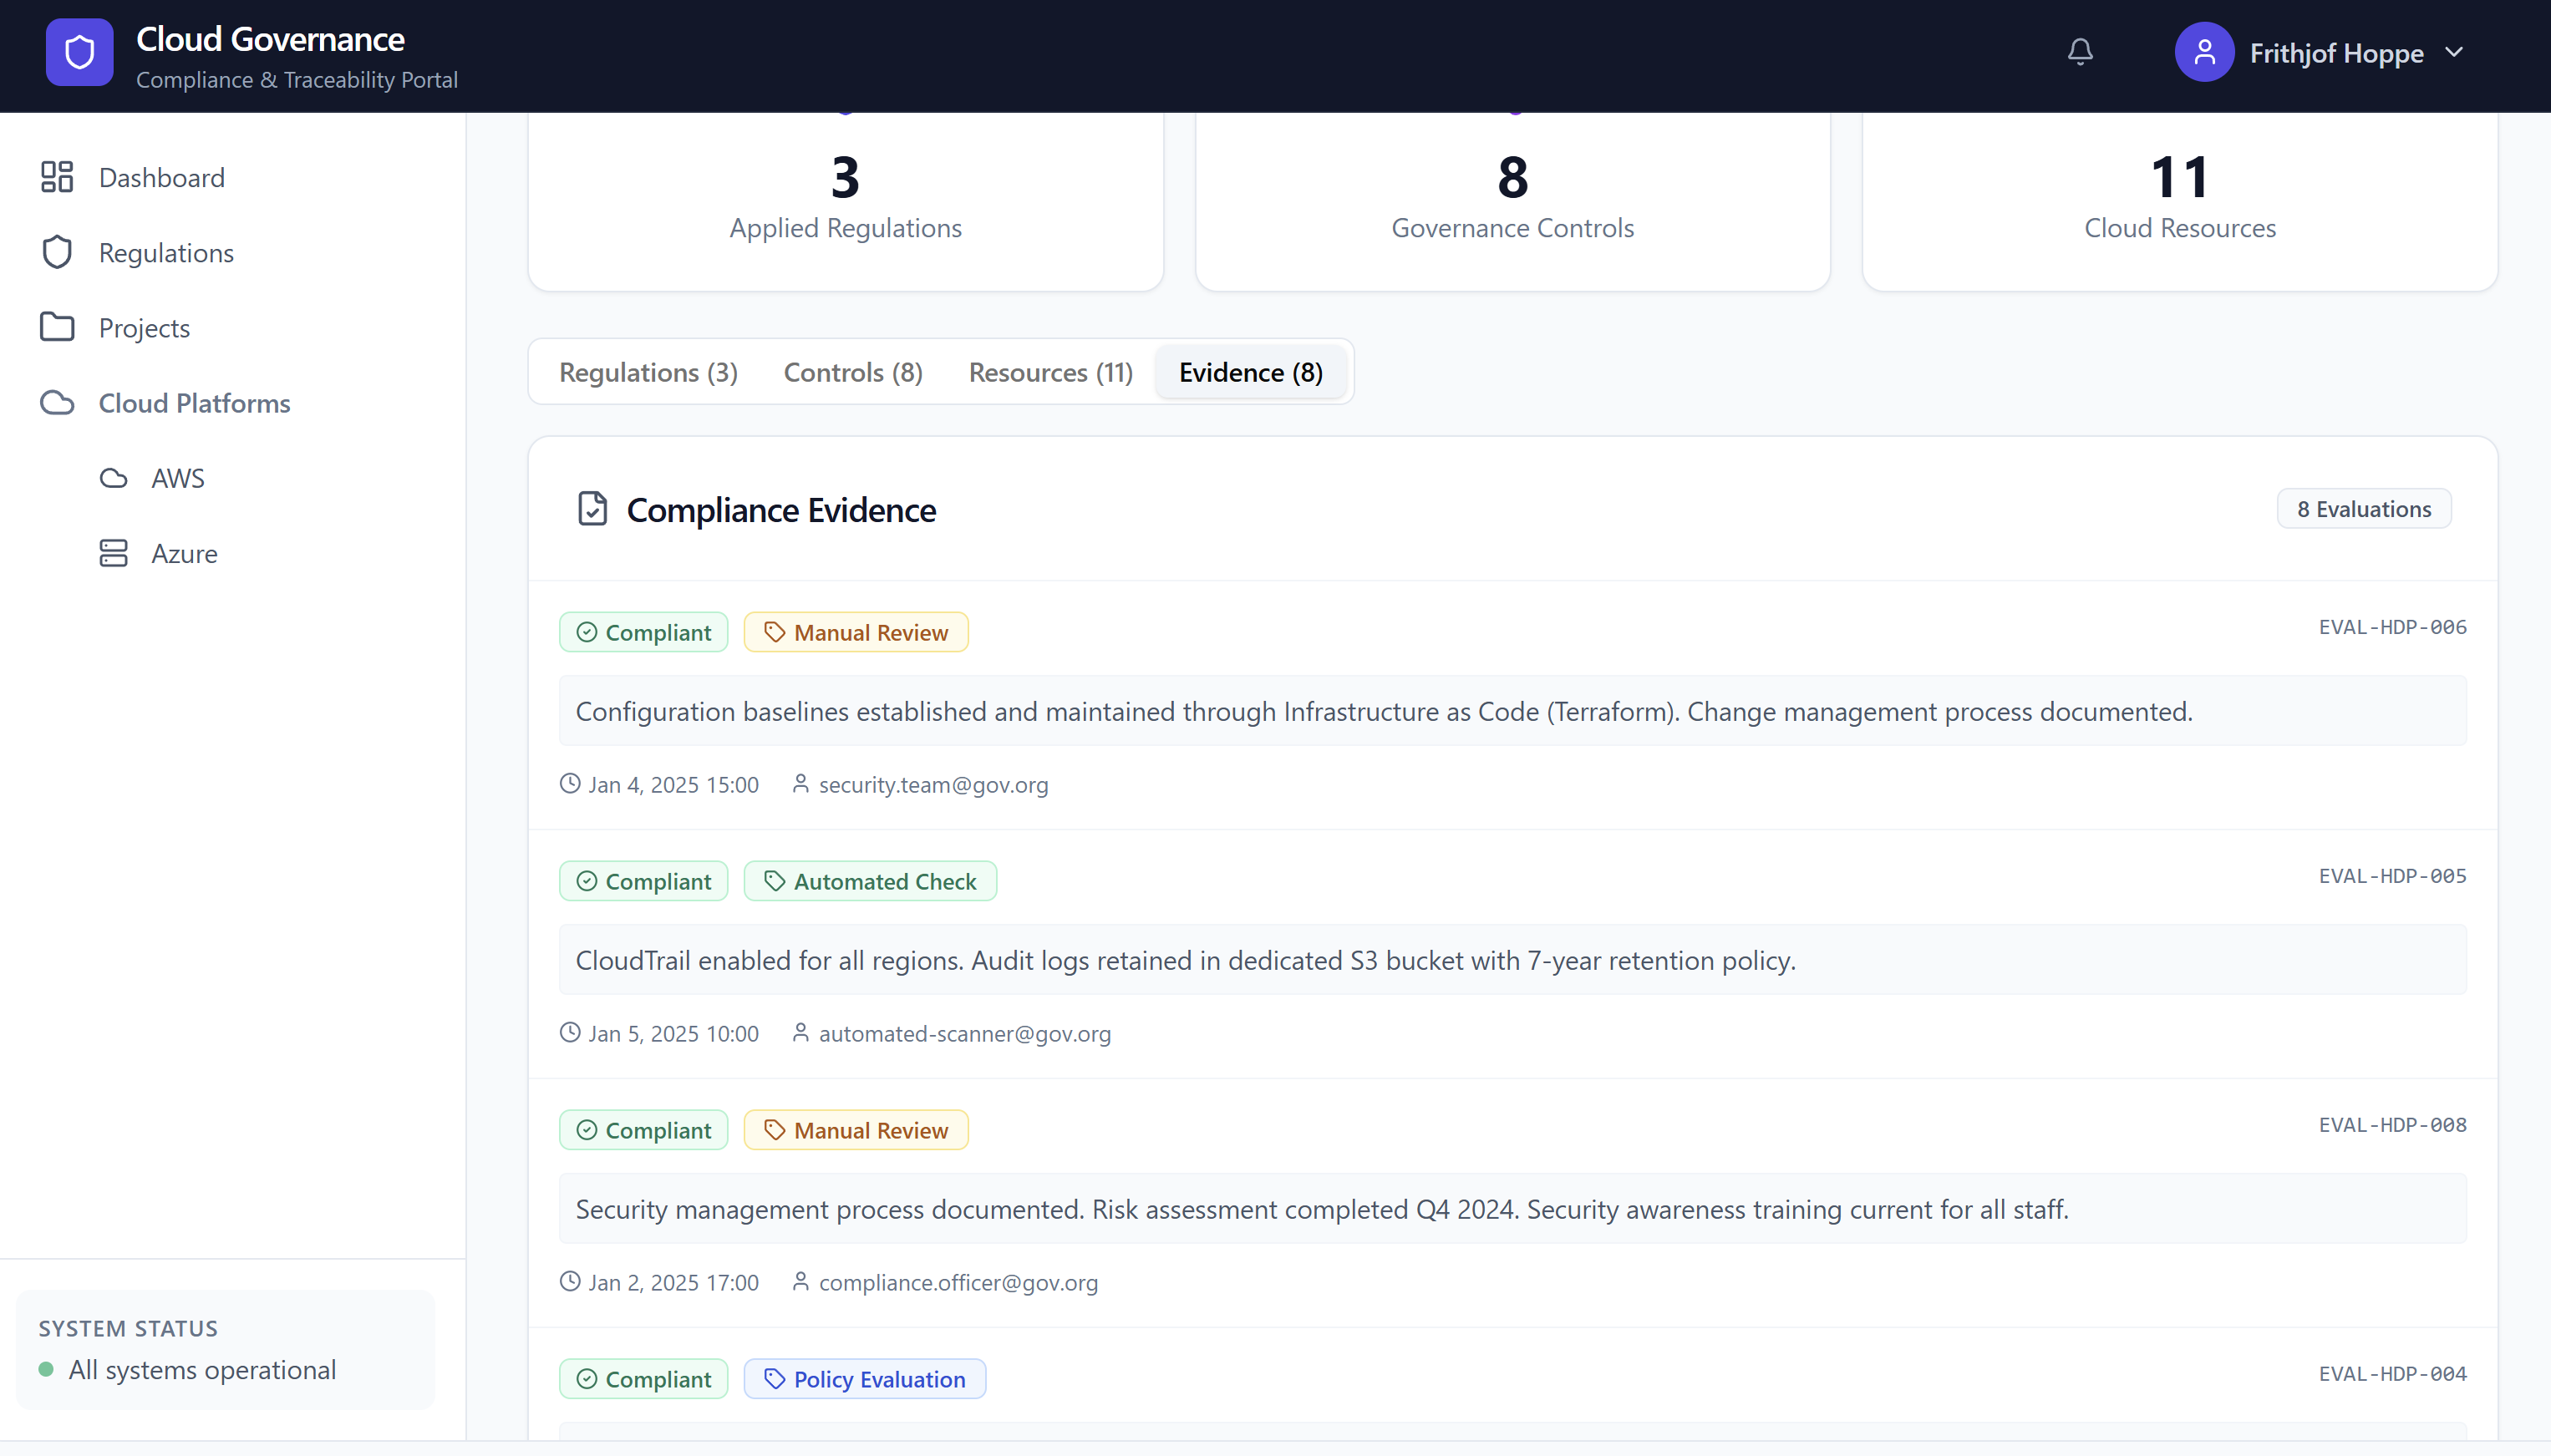
\includegraphics[width=0.8\textwidth]{graphics/ui-prototyp_project_healthcare_view_evidence.png}
    \caption{Detailansicht der beinhalteten Evidence im Beispielprojekt Healthcare}
    \label{fig:methodology-project-healthcare-view-evidence}
\end{figure}

Der \ac{poc} besteht aus den Komponenten in \autoref{fig:methodology-poc-setup}. Das 360-Grad-Cockpit verwaltet mit dem Project Service die Projekte inklusive der zugehörigen Foundations. Der \ac{lz} Provisioning Service provisioniert die Foundations auf den Cloud-Plattformen und hält Referenzen auf die erstellten Cloud Resource Container. Der Hauptanwender des 360-Grad-Cockpit ist der Projektverantwortliche. Das Governance Cockpit verawaltet mit dem Governance Configuration Service die Traceability-Relationship auf welcher Basis der Traceability Service Assessment vornimmt. Der Evidence Service speichert die Artefakte, welche den Stand der Compliance zu einem gewissen Zeitpunkt abbilden. Die Cloud Administration Komponenten provisioniert mit dem \ac{lz} Plattform Configuration Service die Grundinfrastruktur der \ac{lz}. Der Provisioning Service / IaC Execution Layer deckt die Interaktionen inkl. Provisionierung auf den Cloud-Plattformen da. Im \ac{poc} werden lediglich AWS und Azure repräsentativ für weitere grössere Cloud-Plattformen betrachtet.

Um den Fokus auf den genannten Use-Cases zu behalten wird in \autoref{fig:methodology-poc-setup} eine Auswahl getroffen welche Komponenten detailliert implementiert werden. Die grünen Komponenten werden detailliert umgesetzt, um die Funktionalität zu zeigen, die blauen Komponenten werden statisch implementiert da sie sich keinen direkten Bezug zur Funktionsweise der Traceability-Architecture aufweisen.

\begin{figure}[H]
    \centering
    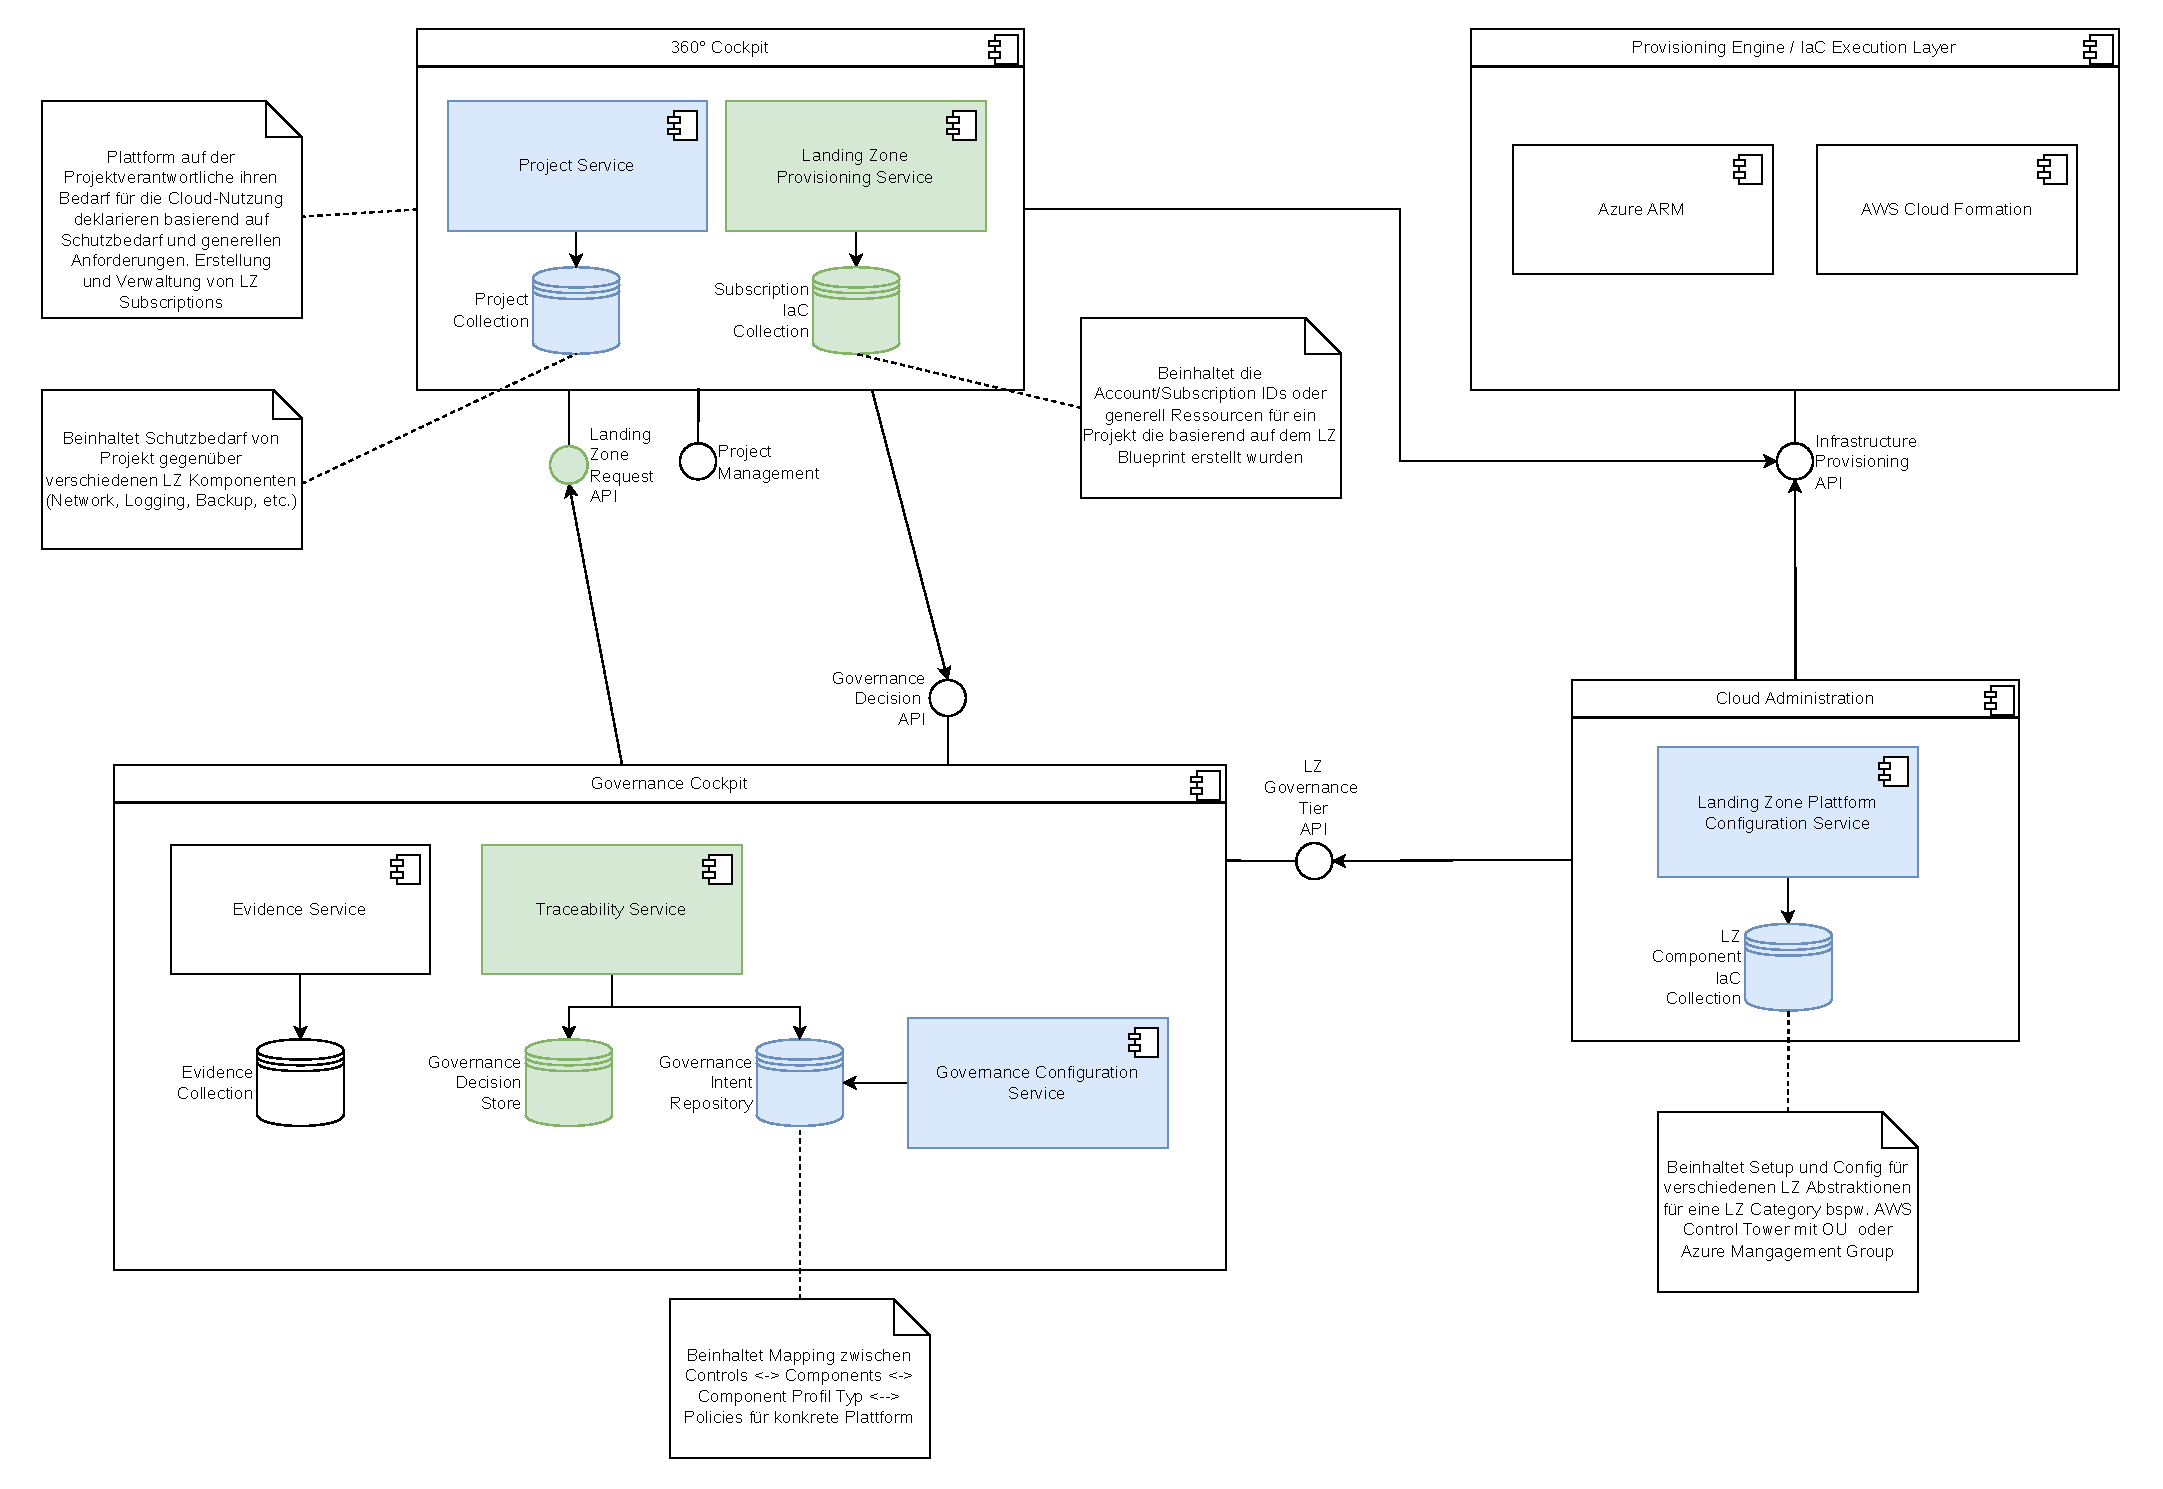
\includegraphics[width=\textwidth]{graphics/ip6-ideation-poc-components.drawio.pdf}
    \caption{Komponenten-Diagramm für den \ac{poc}}
    \label{fig:methodology-poc-setup}
\end{figure}

Im \ac{poc} ist für die Traceability der statisch konfigurierte Inhalte des Governance Configuration Service am relevantesten. Für die implementierte component-cenctric Variante werden in {fig:methodology-poc-traceability-relationship-components} dafür zuerst exemplarische Controls aus der Regulation \ac{si001} gewählt. Die Controls decken absichtlich unterschiedliche regulatorische Gebiete ab, damit eine Zuordnung zu verschiedenen Components in diesem Fall Storage, Network und Compute möglich ist. Nach den Controls werden bereits existieren Policies für die Cloud-Plattformen (Azure und AWS) mittels öffentlicher Dokumentation gesucht und wiederum Component/Component-Profiles zugewiesen. Die Component-Profiles werden im \ac{poc} nicht genauer spezifiziert und dienen lediglich als Veranschaulichung. Für eine produktive Anwendung müsste an dieser Stelle ein Security-Intent für ein Profil definiert werden und basierend auf diesem entsprechend Policies mit Parameter gemapped werden.

\begin{figure}[H]
    \centering
    \centering
    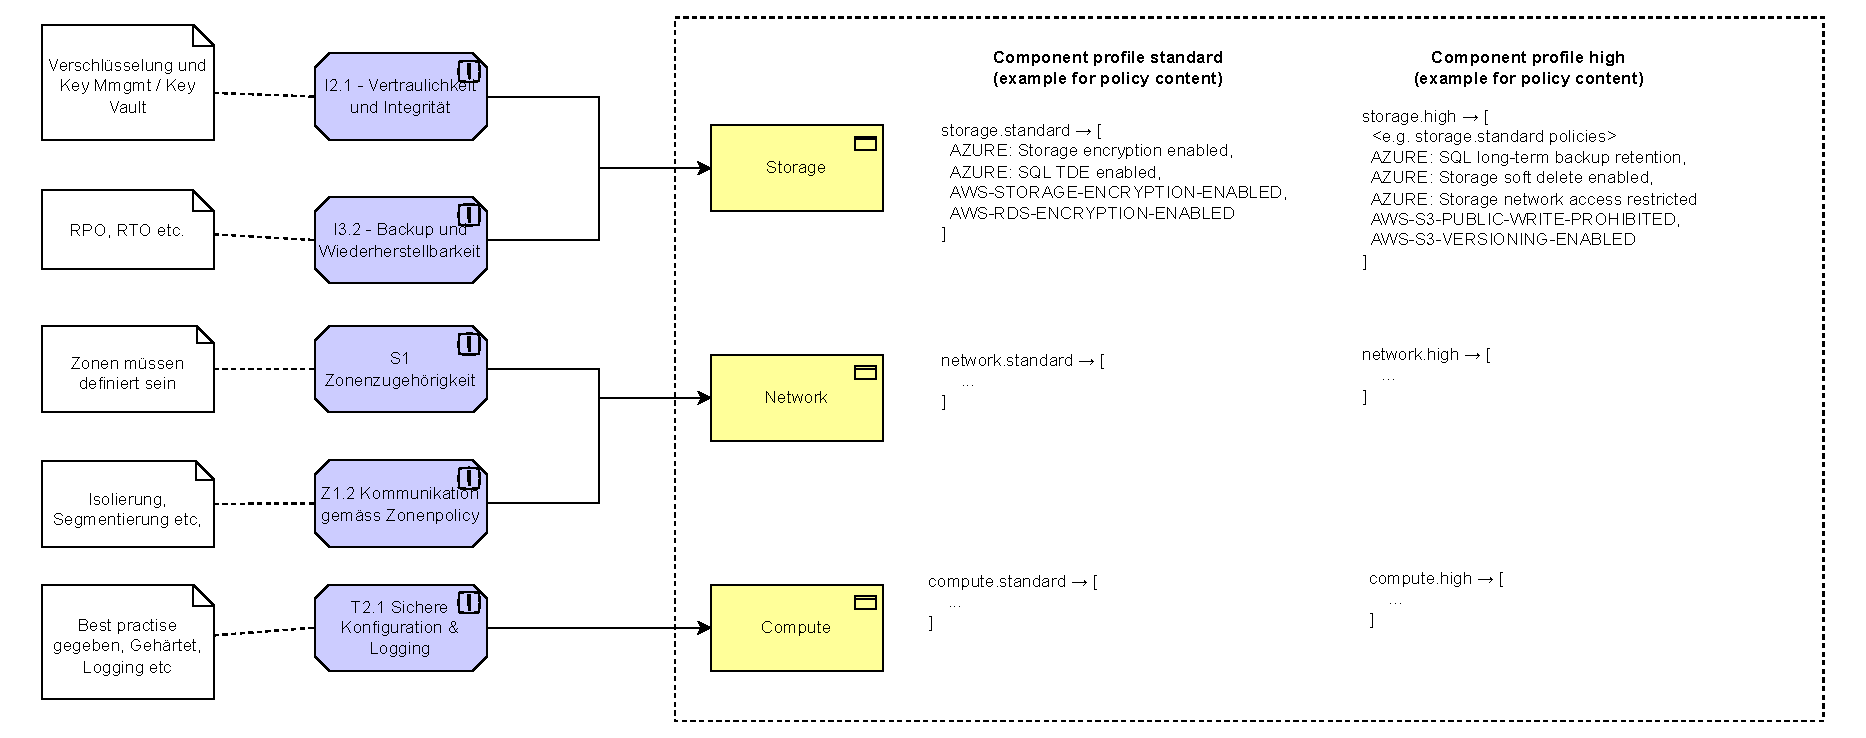
\includegraphics[width=\textwidth]{graphics/ip6-ideation-poc-traceability-components.drawio.pdf}
    \caption{Statische Traceability-Relationship Komponenten für den \ac{poc}}
    \label{fig:methodology-poc-traceability-relationship-components}
\end{figure}